\section{Containers}

\begin{frame}{Importance of Containers}
	\centering
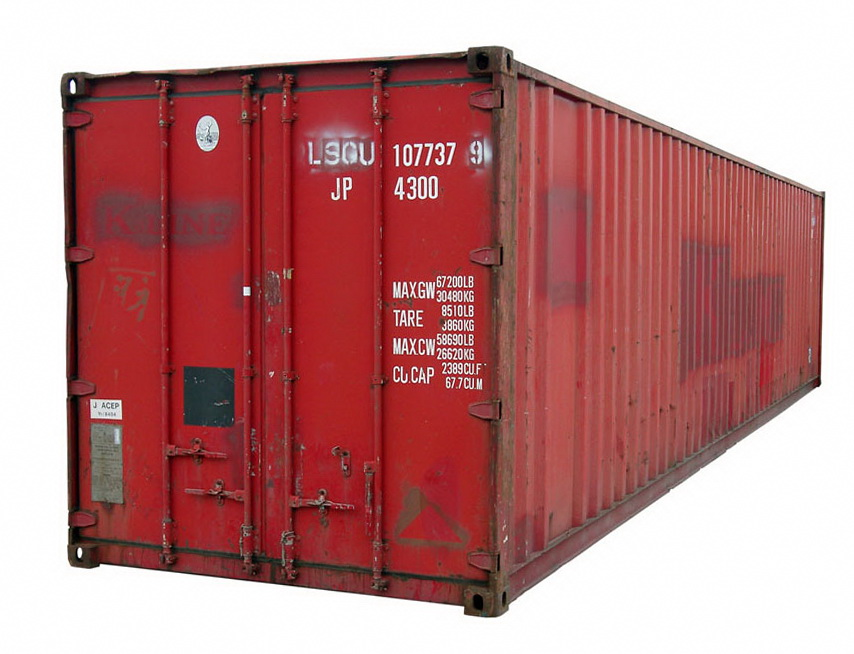
\includegraphics[width=0.7\textwidth]{figures/shipping_container}
\end{frame}

\begin{frame}{Before Containerization}
	\begin{columns}[c]
		\begin{column}{0.5\textwidth}
			\begin{itemize}
				\item Goods had to be loaded and unloaded individually
				
				 \item Inefficient - it was not uncommon to spend more time loading and loading goods than transporting them
				 
				 \item Insecure - goods had be handled by many people, increasing the chance for loss and theft
				 
				 \item Inaccessible - Long distance shipping only available to the wealthy 
			\end{itemize}
		\end{column}
	\begin{column}{0.5\textwidth}
		\centering
	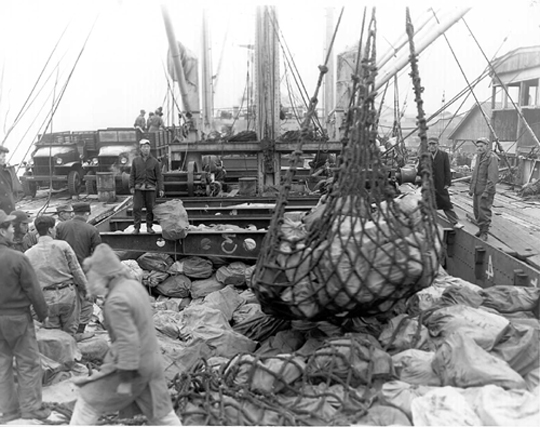
\includegraphics[width=0.85\textwidth]{figures/old_ship_unloading}
\end{column}
\end{columns}
\end{frame}

\begin{frame}{After Containerization}
	\begin{columns}[c]
		\begin{column}{0.5\textwidth}
			\begin{itemize}
				\item Standardized - containers are all the same size and weight allowances
				
				\item Efficient - containers are easy to load and unload and transfer to other modes of transportation
				
				\item Secure - goods may be secured in containers from source to final destination
				
				\item Available - cost effective to ship goods across the world
			\end{itemize}
		\end{column}
		\begin{column}{0.5\textwidth}
			\centering
			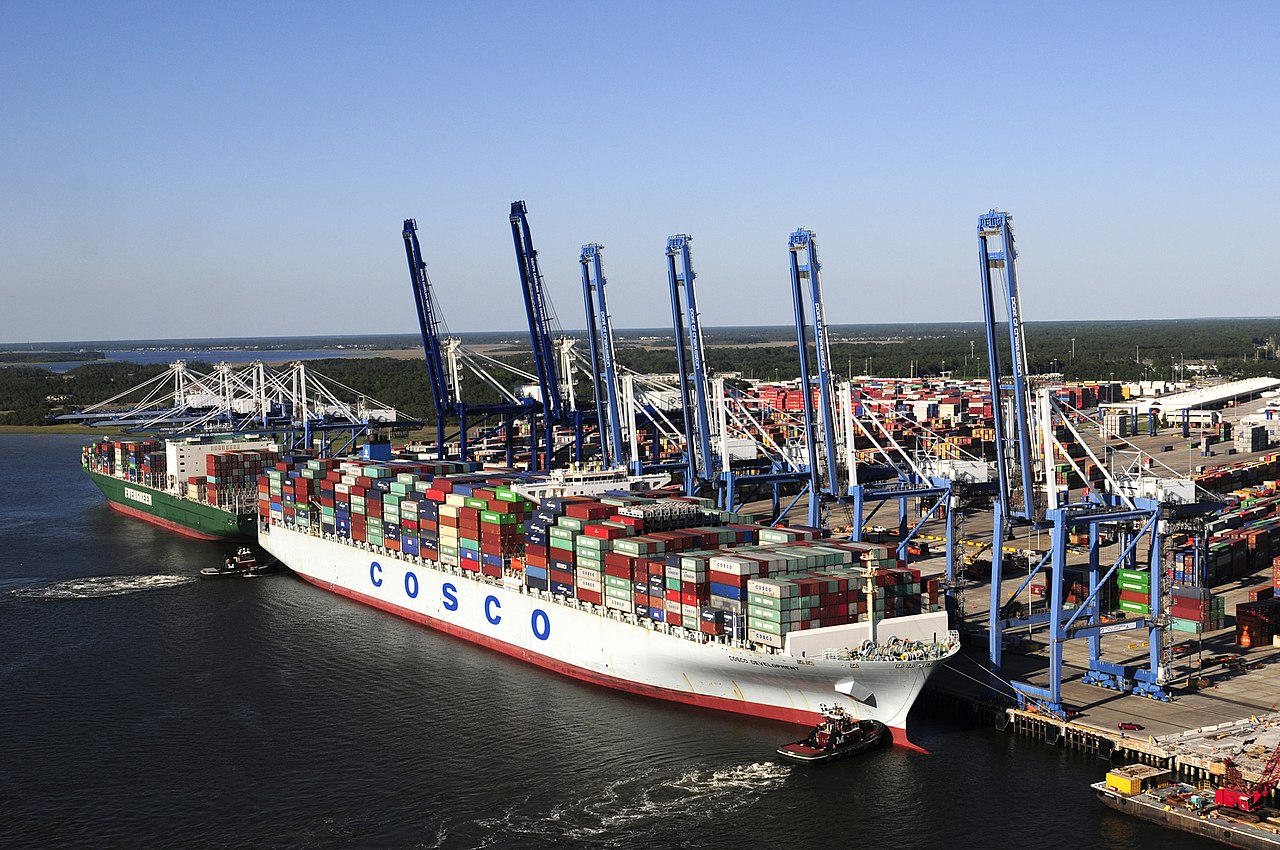
\includegraphics[width=0.85\textwidth]{figures/cargo_ship}
		\end{column}
	\end{columns}
	
\end{frame}

\begin{frame}{What about computing?}
	\begin{itemize}
		\item It's common to run on multiple systems with different requirements
				
		\item We would like to avoid installing the same sets of software again and again
				
		\item We would like other people to run our software without our help
				
		\item  We would like to preserve a known configuration that our software works in
	\end{itemize}
\end{frame}

\begin{frame}{Containers Overview}
	\begin{itemize}
		\item Containers offer the ability to run fully customized software stacks,
		e.g.\ based on different Linux distributions and versions
		\item Containers are not virtual machines, where an entire hardware platform is
		virtualized, rather containers share a common kernel and access to physical
		hardware resources
		\item \href{https://www.docker.com}{Docker} is a popular container platform in
		development and server environments
		\item \href{https://sylabs.io}{Singularity} is a popular container platform in
		HPC environments
		\begin{itemize}
			\item Docker is not directly support on ManeFrame II
			\item Singularity can consume and run Docker containers
		\end{itemize}
	\end{itemize}
\end{frame}

\begin{frame}{Container Benefits}
	\begin{itemize}
		\item \textbf{Performance}: containers can perform at near native performance
		\item \textbf{Flexibility}: install (almost) any software you need
		\item \textbf{Reproducibility}: create complex software environments that are easy to manage and are verifiable.
		\item \textbf{Compatibility}: built on open standards that works on all major Linux distributions
		\item \textbf{Portability}: Build once and run (almost) anywhere
	\end{itemize}
\end{frame}

\begin{frame}{Container Limitations}
	\begin{itemize}
		\item \textbf{Architecture dependent}: Containers are (currently) limited to the same CPU architecture (x86\_64, ARM, etc.) and binary formats
		\item \textbf{Portability}: Requires glibc and kernel compatibility between host and container. Other kernel level APIs may also need to be compatible (e.g. CUDA/GPU drivers, network drivers, etc.)
		\item \textbf{Filesystem Isolation}: paths are (usually) different when viewed from inside or outside of a container
	\end{itemize}
\end{frame}

\begin{frame}{Docker and HPC}
	\begin{itemize}
		\item We don't allow direct Docker use on M2 
		\item Docker's security model is designed to support users "trusted" users running "trusted" containers (e.g. users who can escalate to root access)
		\item Docker is not designed to support scripted / batch based workflows
		\item Docker is not designed to support parallel applications
	\end{itemize}
\end{frame}

\begin{frame}{Singularity Features}
	\begin{itemize}
		\item Containers are a single image file
		\item No root owned daemon processes
		\item User inside containers are the same as users outside the container (no contextual changes)
		\item Supports shared, multi-user environments
		\item Supports HPC hardware such as GPUs and Infiniband networks
		\item Supports HPC applications like MPI
	\end{itemize}
\end{frame}

\begin{frame}{Common Use Cases}
	\begin{itemize}
		\item Converting Docker containers to Singularity
		\item Building and running software that require newer systems and libraries 
		\item Running commercial software binaries that have specific requirements
	\end{itemize}
\end{frame}

\begin{frame}{Singularity Workflow}
	\begin{itemize}
		\item Build your Singularity containers on a local system you have root or sudo access. Alternatively build a Docker container
		\item Transfer your container to M2 or other HPC system. If you used Docker, you will need to convert the image 
		\item Run your Singularity containers
	\end{itemize}
\end{frame}

\begin{frame}{Singularity Options for Mac and Windows}
	\begin{itemize}
		\item Install VirtualBox on your computer
		\item Create an Ubuntu or Red Hat based virtual machine
		\item Install Singularity on the virtual machine. (Note: install the same version the HPC system uses.)
	\end{itemize}
\end{frame}

\begin{frame}{MPI and GPU Accelerated Containers }
	\begin{itemize}
		\item Generally you should try to use the same MPI distribution and Infiniband drivers inside and outside the container
		\item You should use the same GPU drivers and libraries inside and outside the container
		\item You can sometimes mount system GPU settings with the \emph{--nv} option
		\item \textbf{Ask us for help!} Configuration settings are often subtle and may not be obvious from the user environments
	\end{itemize}
\end{frame}

\begin{frame}{Singularity Commands}
	

	\textbf{singularity [options]  \textless subcommand\textgreater   [subcommand options] ...}

   The main subcommands you should know are 
	\begin{itemize}
		\item \textbf{build}: Build your container from a definition file, download an existing container, or convert a container from one format to another (Docker to Singularity)
		\item \textbf{shell}: Spawn an interactive shell session inside your container
		\item \textbf{exec}: Run an arbitrary command inside your container
	\end{itemize}
\end{frame}

\begin{frame}{Singularity Build Script Example}
\begin{listing}[H]
\inputminted{Singularity}{examples/python3.singularity}
\caption{Example Singularity build file that uses Ubuntu 18.04 and Python3 with
package installation via \mintinline{sh}{apt} and \mintinline{sh}{pip}.}
\end{listing}
\end{frame}

\begin{frame}{Building Singularity Container Images}
\begin{listing}[H]
\inputminted{sh}{examples/build_python3_singularity.sh}
\caption{Steps to build a Singularity container image. Note that building
Singularity container images from build scripts on M2 requires permission.}
\end{listing}
\end{frame}

\begin{frame}{Docker Build Script Example}
\begin{listing}[H]
\inputminted{Dockerfile}{examples/python3.dockerfile}
\caption{Example Dockerfile that uses Ubuntu 18.04 and Python3 with package
installation via \mintinline{sh}{apt} and \mintinline{sh}{pip}.}
\end{listing}
\end{frame}

\begin{frame}{Building and Converting Docker Container Images}
\begin{columns}[T]
\begin{column}{0.45\textwidth}
\begin{listing}[H]
\inputminted{sh}{examples/build_python3_docker.sh}
\caption{Building the Docker container off of M2, exporting the container
image, and uploading to M2.}
\end{listing}
\end{column}
\begin{column}{0.45\textwidth}
\begin{listing}[H]
\inputminted{sh}{examples/python3_docker_to_singularity.sh}
\caption{Converting the uploaded Docker container image to a Singularity
container image.}
\end{listing}
\end{column}
\end{columns}
\end{frame}

